
\newpage

% \begin{flushright}
%     \vspace{10cm}
%     \rule{18cm}{5pt}
%     \rule{18cm}{2pt}\vskip1cm
%     \begin{center}
%     \begin{bfseries}
%         \Huge{Explore \& Build a Use Case}\\
%     \end{bfseries}
%     \end{center}
%     \vspace{1cm}
%     \rule{18cm}{2pt}
%     \rule{18cm}{5pt}
% \end{flushright}
\clearpage

\chapter{Final Architecture}
\section{Architecture Diagram}
\begin{figure}[htp]
    \centering
    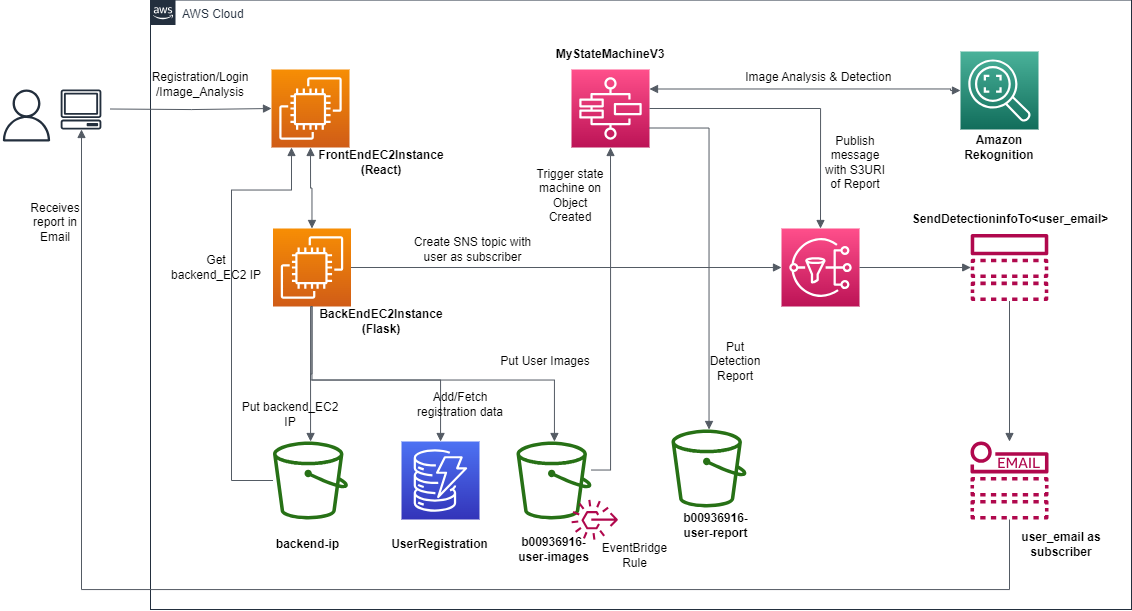
\includegraphics[width=15.5cm]{Chapter_5/arch diag.drawio -v2.png}
    \caption{\textbf{\textit{AWS Architecture diagram of my project (Tool used: draw.io[11])}}}
    \label{fig:my_label}
\end{figure}
The final architecture of the cloud application combines various cloud mechanisms and services to deliver a scalable, efficient, and user-friendly platform for image processing and analysis. The architecture leverages a serverless model for image processing tasks while utilizing other AWS services for data storage and application hosting.

\section{Cloud Mechanisms and Services}
\begin{enumerate}
    \item \textbf{Serverless Architecture}: The core of the application's image processing capabilities is based on a serverless architecture. AWS Lambda is used to execute code in response to image upload events. Lambda functions are responsible for image analysis tasks using Amazon Rekognition. This serverless model ensures cost-efficiency, automatic scaling, and real-time responsiveness.

    \item \textbf{Hosting}: The frontend and backend of the application is hosted on Amazon EC2 instances. These instances serve as web servers, handling user interactions and communication with the serverless components. The choice of EC2 for hosting provides greater control and flexibility over the application's user interface.

    \item \textbf{Data Storage}: The application utilizes Amazon S3 for object storage and Amazon DynamoDB for NoSQL data storage. Amazon S3 is used to store uploaded images, and DynamoDB is used to store user registration data, including user details such as name, email, and password.

    \item \textbf{State Machine}: AWS Step Functions are utilized to orchestrate the image analysis workflow. The state machine coordinates the various steps involved in analyzing the uploaded image using Amazon Rekognition and generating the report.txt file.

    
\end{enumerate}

\section{Programming Languages}
\begin{enumerate}
    \item \textbf{Backend}: The backend of the application is implemented using \textbf{Flask, a Python-based web framework}. Python is chosen for its simplicity, ease of use, and extensive libraries, making it suitable for developing the application's server-side logic and integrating with AWS services.

    \item \textbf{Frontend}: The frontend is developed using \textbf{React.js, a popular JavaScript library} known for its flexibility, component-based structure, and efficient rendering. React.js enables the creation of dynamic and interactive user interfaces, enhancing the user experience.
\end{enumerate}

\section{System Deployment}
The system is deployed to the cloud by utilizing AWS services, provisioned via cloud formation template. The frontend, implemented using React.js, is hosted on Amazon EC2 instances, making it accessible to users through their web browsers. The backend, built with Flask, is deployed on separate EC2 instances to handle user authentication and communication with Lambda functions for image processing.

Lambda functions for image analysis are triggered automatically by image uploads to Amazon S3, which serves as the event source. AWS Step Functions coordinate the image analysis workflow, ensuring a seamless flow of tasks and generating the report.txt file.

Additionally, Docker images are utilized for both the frontend and backend components of the application. These Docker images facilitate the containerization of the application, ensuring consistency and portability across different environments. The Docker images are hosted on public repository in my personal docker account, allowing for easy management and distribution of the application containers.

\section{Comparison of my architecture to the ones taught in lectures}
Upon reviewing the architectures taught in class, my cloud application architecture aligns closely with the "Dynamic Scalability Architecture" and partially incorporates elements from the "Elastic Disk Provisioning Architecture" and the "Redundant Storage Architecture." Let's compare my architecture with these taught architectures:

\subsection{Dynamic Scalability Architecture}
\begin{enumerate}
    \item My application's serverless deployment model with AWS Lambda and Step Functions reflects the dynamic scalability architecture. AWS Lambda allows automatic scaling based on the incoming image processing requests, ensuring efficient resource utilization.[25]
    
    \item \textbf{Justification}: The serverless architecture is well-suited for your application, which involves sporadic image processing tasks. It automatically scales resources up or down based on demand, optimizing costs and ensuring real-time responsiveness.
\end{enumerate}

\subsection{Elastic Disk Provisioning Architecture}
\begin{enumerate}
    \item While my application uses Amazon S3 for object storage, it does not fully align with the elastic disk provisioning architecture, as this architecture typically involves provisioning storage volumes with automatic scaling capabilities.[26]
    
    \item \textbf{Justification}: The usage of Amazon S3 as object storage is appropriate for my application. S3 is inherently elastic and allows me to store and retrieve any amount of data without worrying about provisioning or managing disk volumes. Its pay-as-you-go pricing model makes it cost-effective for variable storage requirements.
\end{enumerate}

\subsection{Redundant Storage Architecture}
\begin{enumerate}
    \item My application's use of Amazon S3 for data storage partly aligns with the redundant storage architecture, as S3 automatically replicates data across multiple availability zones to ensure durability and availability.[27]
    
    \item \textbf{Justification}: Storing data in Amazon S3 provides a level of redundancy as S3 automatically replicates data across multiple geographic locations, making it highly durable and available. This redundancy ensures that your application's data is protected from potential hardware failures.
\end{enumerate}

\subsection{Service-Oriented Architecture (SOA)}
\begin{enumerate}
    \item My cloud application utilizes a Service-Oriented Architecture (SOA) to achieve its functionalities efficiently. The architecture consists of loosely coupled and independent services, each handling specific tasks. AWS Lambda serves as the image processing service, triggered by image uploads to Amazon S3. User registration data is stored in Amazon DynamoDB, representing a separate service. The frontend, developed using React.js, acts as a service for user interface and interactions. The backend, implemented with Flask, handles user authentication and communication with the image processing service. Amazon SNS serves as the notification service, communicating messages to users. [28]
    
    \item \textbf{Justification}: SOA enables a modular and scalable design, enhancing flexibility, reusability, and maintainability. It promotes seamless integration with other services and simplifies updates, ensuring agility and efficient communication among components. Adopting SOA ensures a robust and future-proof architecture for the cloud application.
\end{enumerate}


\section{Conclusion}
My cloud application architecture is well-designed, combining the advantages of serverless computing with EC2 instances for frontend and backend hosting. It effectively leverages the dynamic scalability architecture with AWS Lambda and Step Functions for image processing tasks. The usage of Amazon S3 for object storage ensures redundancy and data durability, even though it does not strictly align with the elastic disk provisioning architecture. Overall, my choices are justified, as the architecture optimizes performance, cost, and user experience for the image analysis application.



\newpage

\comment{
\chapter*{Revision History}

\begin{center}
    \begin{tabular}{|c|c|c|c|}
        \hline
	    Date & Version & Description & Author\\
        \hline
	     04-Mar-2021 & 1.0 & Interaction Diagram Document - Initial Release. & All\\
        \hline
	    %31 & 32 & 33 & 34\\
        % \hline
    \end{tabular}
\end{center}




\newpage
\tableofcontents
}

\comment{
\chapter{Interaction Diagram}
\begin{figure}[htp]
    \centering
    \includegraphics[width=17.5cm]{04 - Interaction Diagram/Quiz Application-2.png}
    \caption{\textbf{\textit{Login functionality - Interaction diagram}}}
    \label{fig:my_label}
\end{figure}

\begin{figure}[htp]
    \centering
    \includegraphics[width=17.5cm]{04 - Interaction Diagram/Quiz Application-1.png}
    \caption{\textbf{\textit{Quiz Application - Interaction diagram }}}
    \label{fig:my_label}
\end{figure}
}